\documentclass[10pt,letterpaper]{article}
\usepackage[latin1]{inputenc}
\usepackage{indentfirst}
\usepackage{amsmath}
\usepackage{amsfonts}
\usepackage{amssymb}
\usepackage{hyperref}
\usepackage{listings}
\usepackage{pdflscape}
\usepackage{geometry}
\usepackage{array}

\usepackage{todonotes}

\DeclareMathOperator*{\argmax}{arg\!max}

\author{Andrew Price}
\title{Planar Segmentation of Multiview RGB-D Image Sets using Markov Chain Monte Carlo }

\begin{document}
\maketitle

\section{Abstract}
	As techniques for reconstructing 3D scenes have progressed beyond purely geometric modelling, attention has now shifted to techniques for understanding the content of these captured scenes. An important intermediate step towards this goal is to be able to segment different objects in the environment from one another, so that recognition can be performed on manageable and consistent components of the captured 3D world. With this objective in view, one possible first step is to begin by first segmenting the world into geometric primitives, in this case planes. This paper presents a method for applying the Swendsen-Wang Markov Chain Monte Carlo approach to simultaneously compute the optimal segmentation for a set of RGB-D images.
		
\section{Introduction}
	Any introduction to a discussion on modern 3D image segmentation or reconstruction ought to begin with an acknowledgement of the impact of consumer RGB-D cameras like the Microsoft Kinect and its brethren from Asus and PrimeSense. Following the Kinect's release in late 2010, there has been an explosion of academic, commercial, and hobbyist applications for the relatively inexpensive devices, spanning such diverse topics as simultaneous localization and mapping, additive manufacturing, visual servoing, and the original purpose of novel user interfaces. Thus, the benefits of developing and extending algorithms that operate on these types of RGB-D data must be readily apparent to the reader.
	
	Much of this research has focused on methods of reconstructing an environment geometrically, first using sparse, point-based methods, then moving more towards volumetric dense methods.
	\todo[inline]{Finish brief history.}
	
\section{Related Work}
	Myriad approaches have been proposed for the 3D image segmentation problem, including RANSAC-based model fitting, region growing, difference of normals, and graph cut methods, with many variations and combinations of these themes. For a general overview of segmentation methods applied to LIDAR captures, the reader is referred to \cite{douillard2011segmentation}. 
	
	For the similar problem of segmenting point clouds derived from colored stereo images, graph cuts have been shown to be effective for segmentation(\cite{bleyer2005graph}).

	
	We wish to strike out in a somewhat different direction from the main branch of research in this area in a couple of different ways. First, we wish to avoid becoming trapped in a local convergence basin, a common limitation of greedy segmentation algorithms. To accomplish this, we employ a modified version of the Markov chain Monte Carlo method described by \cite{swendsen1987nonuniversal}, generalized to arbitrary probability densities by \cite{barbu2005generalizing}, and applied to RGB-D images by \cite{Erdogan12crv}. Such MCMC methods have proven relatively popular for reconstructing surfaces, as shown in \cite{tu2002image}, \cite{qiu2009jump}, and 	\cite{dick2002bayesian}.
	
	Second we choose to perform the segmentation simultaneously on the individual images, rather than fusing all of the images into a single point cloud or volume model. This allows the sampling algorithm to operate directly on the data as it was captured, rather than operating on an aggregated or fused model generated from many separate images.
	
	
	
	\todo[inline]{Mention papers discussed in previous.}
\cite{metropolis1953equation}



\section{Procedure}

\subsection{Problem Definition: Graph Partitioning}

	Before moving on to the specifics of the multiview RGB-D segmentation, we begin by clarifying the more general graph partitioning problem. We define a graph $G<V,E>$ containing vertices $V=\{v_1,v_2,\ldots,v_M\}$ and edges $E$, where each vertex $v_j$ represents an atomic region in an image, or "superpixel". We now wish to find a partition $\pi_n=(V_1,V_2,\ldots,V_n)$ that correctly assigns atomic regions  $v_{j_s}\in{V_j}$. A partition is an assignment of each edge $e_{s,t}$ in graph $G$ to either "on" or "off". An atomic region must exist uniquely in a segment, that is, $\bigcup_{i=1}^{n}V_i=V$ and $V_i\bigcap{V_j}=\emptyset,\forall{i}\neq{j}$.
	
	Additionally, we wish to fit a parameterized model to each segment $V_i$. The full model assigned consists of a model family $l\in{L}$,  $L=$\{planar, cylindrical, spherical, spline, etc.\}, that describes the nature of the underlying surface, as well as a parameterization $\theta_i$ $i=1,2,\ldots,n$ containing the coefficients for the given model type. For the plane model (used exclusively in this paper), these are the coefficients from the plane equation $ax+by+cz=d$. We can combine these components into a full model description $c_i=(l_i,\theta_i)$ $i=1,2,\ldots,n$ that is analogous to the graph color assignment in \cite{swendsen1987nonuniversal}.
	
	Armed with descriptions of both which superpixels are associated with one another and what model describes these segments, we can construct a full world description $W=(n,\pi_n,c_1,c_2,\ldots,c_n)$. The  This is the function we are trying to optimize via $W^*={\argmax}_{W\in\Omega} P(I|W)P(W)$. For our problem, the search space $\Omega$ is very large, with $\Omega=\bigcup_{n=1}^{|V|}\{\Omega_{\pi_n} \times\Omega_{l}^n \times\Omega_{\theta_1} \times\Omega_{\theta_2},\ldots, \times\Omega_{\theta_n}\}$.
	
	
	
	
	
	In order to accelerate the convergence
	\cite{barbu2005generalizing}
	discriminative probabilities
	proposal density
	rho

\subsection{Image Graph Generation}
	In order to generate an initial oversegmentation and adjacency graph for each image in the set, we adhere closely to the work presented in \cite{Erdogan12crv}. We employ a modified version of the graph-cut algorithm presented in \cite{felzenszwalb2004efficient}, adding factors for both color and depth components in the image.
\begin{equation}
w_{i,j}=\alpha w_C + \beta w_D + \gamma w_S
\end{equation}
\begin{align*}
w_C&=\sqrt{(r_i-r_j)^2+(g_i-g_j)^2+(b_i-b_j)^2+(z_i-z_j)^2} \\
w_D&=abs(z_i-z_j) \\
w_S&=\sqrt{(u_i-u_j)^2+(v_i-v_j)^2} \\
\end{align*}
	\todo[inline]{summarize Can's paper here}
	Next, we compute a set of properties, $\rho$, for each superpixel. These properties will help us to generate more efficient proposal densities when we wish to sample from the graph configurations. We achieve this by incorporating a discriminative probability $q_e$ for each edge $e\in{E}$ determined by the following equation: 
\begin{equation}
	q_e=P(\mu_e=on|\rho_s,\rho_t)=e^{\|w_\rho\odot(\rho_s-\rho_t)\|^2\frac{T}{2}}
	\label{eq:edgeProb}
\end{equation}
where $\mu_e$ is a random binary variable following a Bernoulli distribution and representing the state of an edge in a given sample, $w_\rho$ is a weight vector to account for the various units used (neighboring pixel distances might be on the order of 0.01m, while color differences might be on the order of 10 units), $\odot$ represents element-wise vector multiplication, and $T$ is a temperature factor.

\subsection{World Graph Generation}
	Having generated a weighted superpixel adjacency graph for each image $I_t$ in the input sequence, we now wish to create a world graph $G'_t$ incorporating each individual image graph $G_t$ as a subgraph. $G'$ contains all vertices representing the superpixels, i.e., $V'_t=V'_{t-1}{\bigcup}V_t$. Additionally, this global graph contains all original edges, plus edges that we will add to relate the individual frames to each other, $E'_t=E'_{t-1}{\bigcup}E_t{\bigcup}E(\rho'_s,\rho_k)$,
 $s=1,2,\ldots,\sum_{\tau=1}^{t-1}{N_\tau}$, 
 $K=1,2,\ldots,N_t$.
	The edge generating function $E(\rho'_s,\rho_k)$ is a thresholded version of equation \ref{eq:edgeProb}, where edges are only added if $q_e>q_0$, where $q_0$ is some experimentally determined threshold value.
	
	 The adjacency graph for the image at time $t$
 The world graph incorporating all images up to time $t$
 Set of vertices at time $t$



Set of edges at time $t$ 
\subsection{World Graph Sampling}
	An initial partition $\pi_0$ is achieved by turning off edges in the graph according to edge weights $q_e$. The connected components following this operation are the initial segments $\{V_1,V_2,\ldots,V_n\}$. For each of these segments, we compute a best fit surface with parameters $\theta$. The probability of the full segmentation is \todo[inline]{P(pi)}

	We wish to now sample this graph-based configuration space in proportion to the posterior probability density. As shown in  \cite{metropolis1953equation}, this can be achieved even with an unknown posterior function by introducing an acceptance ratio $a$ for a new proposed state as $a=\frac{P(x')}{P(x_t)}$, where $x'$ is a proposed state and $x_t$ is the current state. Proposed states producing $a\geq 1$ are accepted automatically, while others are accepted with probability $a$.
	
	The discriminative probabilities $q_e$ on each edge form the basis for the proposal density for generating new $x'$s. Algorithmically, this is implemented by randomly selecting a superpixel and recursively growing the region probabilistically according to the edge weights.

\begin{equation}
\alpha(S^{A}\rightarrow S^{B})=\frac{\prod_{e\in E(C^{*},V_{1}-C^{*})}(1-q_{e})\, q(V_{1}|C^{*},S^{B})\, p(S^{B}|Z)}{\prod_{e\in E(C^{*},V_{2}-C^{*})}(1-q_{e})\, q(V_{2}|C^{*},S^{A})\, p(S^{A}|Z)}\label{eq: acceptanceRatio}
\end{equation}

\begin{eqnarray}
\frac{p(S^{B}|Z)}{p(S^{A}|Z)} & = & \frac{P(S^{B})\prod_{S_{i}\in S^{B}}P(S_{i}|Z_{i})}{P(S^{A})\prod_{S_{j}\in S^{A}}P(S_{j}|Z_{j})}\nonumber \\
 & = & \frac{P(S_{1}^{B}|Z)P(S_{2}^{B}|Z)}{P(S_{1}^{A}|Z)P(S_{2}^{A}|Z)}\label{eq:jumpProb}
\end{eqnarray}


	$I_t$ RGB-D Image at time $t$ This represents the stream of images to be segmented

$q_e=P(\mu_e=on|c_i,c_j)$ $e\in{E}$ Discriminative probability on edge $e$. $\mu_e$ is a binary random variable following a Bernoulli distribution and describing the probability of two adjacent vertices in $G'_0(t)$ being connected in a given step.
$E'_t(\pi)\subset{E'_t}$ Set of edges turned on for partition $\pi$ at time $t$
\section{Results}

\cite{sturm12iros}
\begin{figure}[here]
\begin{center}
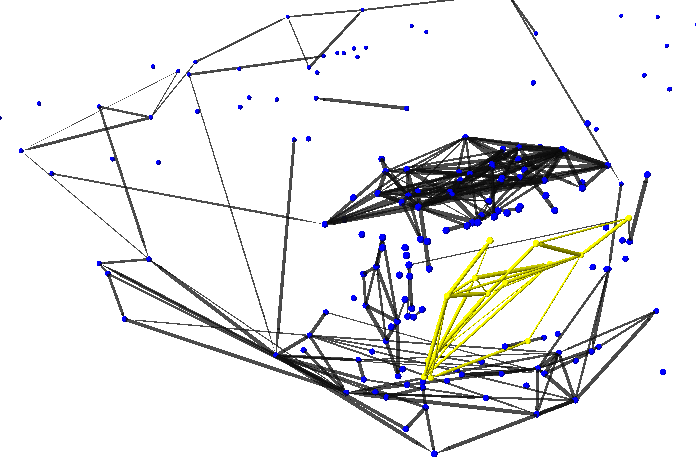
\includegraphics[width=.9\linewidth]{graph1.png}
\end{center}

\caption{3D adjacency graph with one S-W cut highlighted.}
\label{fig:highGraph}
\end{figure}

\section{Conclusions}

\bibliography{references}
\bibliographystyle{unsrt}

\end{document}